\subsubsection*{\underline{\textsc{\Large Child of Abruhan Cultist}}}
\noindent\emph{Medium humanoid elf, any non-good alignment} 

The \emph{Children of Abruhan} are a cult of fanatic believers in the revival of the Abruhan empire. They are responsible for the abductions around the city of Aleytheas. They are seeking to find the bloodline of the one that will revive Uhanos, god of the Abruhani people. 

\noindent\rule{0.5\textwidth}{0.5pt}

\noindent\textbf{Armor Class}: 13 (leather armor)

\noindent\textbf{Hit Points}: 33 (6d8 + 6)

\noindent\textbf{Speed}: 30 ft.

\noindent\rule{0.5\textwidth}{0.5pt}
\begin{table}[H]
	\begin{tabular}{cccccc}
		\textbf{STR} & \textbf{DEX} & \textbf{CON} & \textbf{INT} & \textbf{WIS} & \textbf{CHA} \\
		11 (+0) & 14 (+2) & 12 (+1) & 10 (+0) & 13 (+1) & 14 (+2) \\
	\end{tabular}
\end{table}
\noindent\rule{0.5\textwidth}{0.5pt}

\noindent\textbf{Skills}: Deception +4, Persuasion +4, Religion +2

\noindent\textbf{Senses}: darkvision 60 ft., passive Perception 11

\noindent\textbf{Languages}: Common, Elvish, Abruhani Elvish

\noindent\textbf{Challenge}: 2 (450 XP)

\noindent\rule{0.5\textwidth}{0.5pt}

\noindent\textbf{Dark Devotion}: The child of Abruhan has advantage on saving throws against being charmed or frightened.

\noindent\textbf{Spellcasting}: The child of Abruhan is a 4th-level spellcaster. Its spellcasting ability is Wisdom (spell save DC 11, +3 to hit with spell attacks). They have the following cleric spells prepared:

\textbf{Cantrips}: \emph{\underline{light}} (1 action, touch, 20 ft. bright light around an object), \emph{\underline{sacred flame}} (1 action, 60 ft., 1d8), \emph{\underline{thaumaturgy}} (1 action, 30 ft., manifests a minor wonder, a sign of supernatural power, within range)

\textbf{1st Level (4 slots)}: \emph{\underline{command}} (1 action, 60 ft., speak a one-word command to a creature), \emph{\underline{inflict wounds}} (1 action, touch, 3d10 necrotic damage), \emph{\underline{shield of faith}} (1 bonus action, 60 ft., +2 AC to the target)

\textbf{2nd Level (3 slots)}: \emph{\underline{hold person}} (1 action, 60 ft., target must succeed on a Wisdom saving throw or be paralyzed for the duration), \emph{\underline{spiritual weapon}} (1 action, 60 ft., create a floating, spectral weapon that deals 1d8 + 3, can move the sword as a bonus action)

\noindent\rule{0.5\textwidth}{0.5pt}

\noindent\textbf{ACTIONS}

\noindent\textbf{Multiattack}: The fanatic makes two melee attacks.

\noindent\textbf{Dagger}: Melee or Ranged Weapon Attack: +4 to hit, reach 5 ft. or range 20/60 ft., one creature. Hit: 4 (1d4 + 2) piercing damage.

\begin{center}
	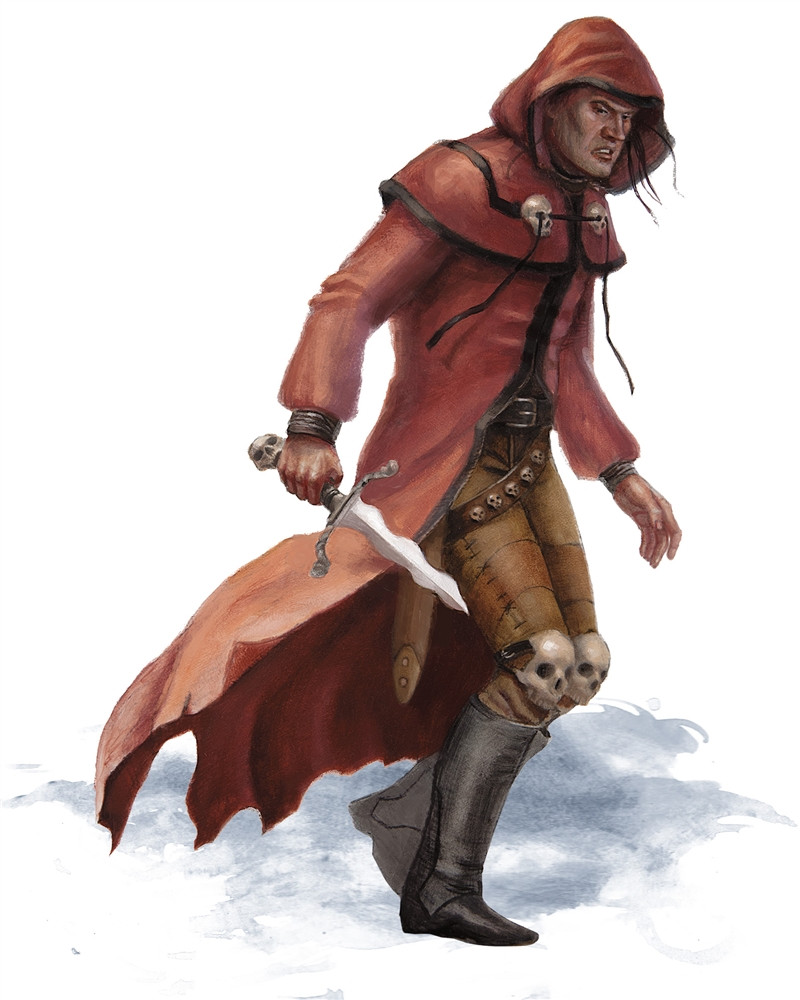
\includegraphics[width = 0.3\textwidth]{child-of-abruhan-cultist}
	
	\emph{Child of Abruhan Cultist}
\end{center}